\documentclass[a4paper]{article}


%analysis to do

%decide if we should set a fixed window that we look at for all sets

% check the degree of multivalyes. UD says: "It is possible to declare that a feature has two or more values for a given word: Case=Acc,Dat. The interpretation is that the word may have one of these values but we cannot decide between them. Such multivalues should be used sparingly. They should not be used if the value list would cover the whole value space, or the subspace valid for the given language. That would mean that we cannot tell anything about this feature for the given word, and then it is preferable to just leave the feature out." 
% discuss: "Not mentioning a feature in the data implies the empty value, which means that the feature is either irrelevant for this part of speech, or its value cannot be determined for this word form due to language-specific reasons." https://universaldependencies.org/u/overview/morphology.html



% Unicode
%\usepackage[utf8]{inputenc}
\usepackage{hyperref}
\hypersetup{
	unicode,
%	colorlinks,
%	breaklinks,
%	urlcolor=cyan, 
%	linkcolor=blue, 
	pdfauthor={Author One, Author Two, Author Three},
	pdftitle={A simple article template},
	pdfsubject={A simple article template},
	pdfkeywords={article, template, simple},
	pdfproducer={LaTeX},
	pdfcreator={pdflatex}
}

\usepackage{booktabs}
\usepackage{multirow}
\usepackage{placeins}
\usepackage{natbib}
% Theorem, Lemma, etc

\usepackage{graphicx, color}
\graphicspath{{latex/fig/}}

% Author info
\title{Using annotated corpora to explore morphological information}
\author{Hedvig Skirgård$^1$ \& Stephen Francis Mann$^1$}

\date{
	$^1$Department of Linguistic and Cultural Evolution, Max Planck Institute for Evolutionary Anthropology, Leipzig, Germany\\%
%	\today
}

\begin{document}
	\maketitle
	
	\begin{abstract}
    The emergence of annotated corpora collections in many different languages opens up new avenues for research in linguistic typology which take into account more nuances of language use.
    In this paper, we use the morphology annotations in the Universal Dependencies datasets (UD) to quantify the information carried by morphological features.
    We propose an approach founded in information theory which focusses on how surprising a certain morphological annotation is given a token's lemma.
    This metric is sensitive to how the morphological annotations are distributed in the data.
    For example, if the tokens of certain lemma have the value IMP for ASPECT 95\% of the time and otherwise PERF, then ASPECT is less informative than if the distribution was 50/50.
    We use these proportions to calculate how surprising the morphological annotation for a given token is and use this to measure overall how much information is carried by morphology in different UD datasets.
    We find that languages vary in how much information is encoded in morphology and that the variation correlates moderately with measurements of fusion, which is a metric that has been used to quantify ``linguistic complexity''.
    We argue that measurements such as the one presented in this paper makes it possible to test more specific hypotheses of ``linguistic complexity'', such as informational load distribution of different parts of language and even non-linguistic domains.
    We also discuss possible modifications to the approach (generalising over part-of-speech or other categories instead of lemma) and shortcomings (reliability of morphological annotation, null-marking, conditional probabilities etc). 
	
    \noindent\textbf{Keywords:} morphology, Universal Dependencies, corpora, information theory, surprisal
	\end{abstract}
\newpage
\tableofcontents


\newpage
\section{Introduction}
Do some languages necessarily encode more information than others?
All languages can express all concepts, albeit in different ways and perhaps at varying length. 
There may not be a word for the German expression ``schadenfreude'' in all languages, but we can approximate the meaning (though it may take us several words - even several clauses). 
Grammar is the set of rules of a language that determine how to put units together, and what has to be specified. 
``grammar [...] determines those aspects of each experience that must be expressed'' \citep[132]{boas1938language}. 
Languages differ in their grammar, which means they also differ in what ``must be expressed''. 
For example, some languages have pronoun systems with a distinction between inclusive and exclusive ``we'' (e.g. S\={a}moan l\={a}tou / m\={a}tou). 
While the English language does not have such a grammatical distinction in its pronoun system, the information can be expressed optionally in English (e.g. ``we, you and I, are going''). 
In English, this information is optional and the utterance can be left ambiguous between including the hearer or not without being ungrammatical. In S\={a}moan, the distinction is made every time ``we'' is expressed. 
The grammar of S\={a}moan entails a higher degree of information specificity in this particular regard. There is other information that English grammar specifies which S\={a}moan does not, such as masculine / feminine gender on 3rd person pronouns.

We can compare languages in terms of how much specific information their grammars determine. In this paper we investigate this using cross-linguistic corpora, and we also study how those distinctions are used in terms of their frequency. For example, it is possible that a particular grammatical distinction exists in a language such that there are two alternatives, but 90\% of the time speakers just use one alternative. Such a distinction is less informative than one that shows more variation between the alternatives frequency.

Informational distinctiveness in grammar is one of the concepts that is covered by the term ``language complexity''. In this paper we give a brief overview of research on ``language complexity'' and where this study is situated.


\section{Background}
\subsection{Language complexity''}
%Measuring information
Language complexity has fascinated linguists and other scholars for a long time. There are many theories, primarily relating language complexity to contact languages \citep{mcwhorter_200} and population size and/or proportion of non-native speakers (inter alia \citet{wray2007consequences, dahl2004growth, lupyan2010language, bentz2013languages, bentz2015adaptive, raviv2019larger, koplenig2019language, shcherbakova2023societies}). Broadly one can characterise the field of research as being concerned with how and under what conditions languages acquire more complexity than would seem necessary for pure information transmission and how such complexity can be lost.
Language complexity can be operationalised into different specific measurements. 
Some of these measurements are correlated \citep{bentz2016comparison}, however as they map onto different theories of causation and phenomena in the languages themselves they can be significantly different (cf. \citet{lupyan2024cautionary}). 
Table \ref{tab:complex_metrics} gives an overview of several different ways of measuring language complexity. Note that for some of the measurements, there are instantiations using typological survey of grammars or language corpora.


\begin{table}[h]
    \centering
    \begin{tabular}{p{3cm}p{5cm}p{2.5cm}p{3cm}p{2cm}}  % Adjust column alignment as needed
        \toprule
        \textbf{Metric} & \textbf{Description} & \textbf{Data source} & \textbf{Studies (selection)} \\ 
        \midrule
       \multirow{2}{3cm}{boundedness/fusion}   & \multirow{2}{5cm}{how much grammatical material is morphologically bound to verb/noun/other Part-of-Speech (c.f. isolating/agglutinating/ synthetic) } & typological survey of grammars & \cite{grambank_release}; \cite{shcherbakova2023societies} \\ 
        \cmidrule{3-4}
         &  & language corpora \\ 
         \midrule
        type-token-ratio (TTR) & how many unique words in relation to all words (more morphology = more unique words) & language corpora &  \cite{kettunen2014can}\\ 
               \midrule
     \multirow{2}{3cm}{information/ informativity}     & \multirow{2}{5cm}{how much information is expressed (via grammar/words)} & typological survey of grammars & \cite{shcherbakova2023societies} \\
       \cmidrule{3-4}
      &  & natural language corpora \\    \midrule
redundancy  & how much information is repeated &&  \cite{leufkens2023measuring}\\    \midrule
systematicity/ transparency  & the degree of consistency of form to meaning patterns && \cite{raviv2019larger}; \cite{hengeveld2018transparent} \\    \midrule
regularity & the consistency of rules, for example in paradigms & & \cite{round2022cognition}\\    \midrule
compositionality  & The extent to which the meaning of larger units is built from the meanings of smaller parts &  &\cite{wray2007consequences} \\    \midrule
compressibility  & how much a computer algorithm can compress language material & & \cite{juola1998measuring} \\    \midrule
ease of LLM-learning  & &how easy is it for an LLM to learn the language & \cite{koplenig2023languages}  \\    \midrule

prediction accuracy  & how accurately the next item can be predicted && \cite{frank2011insensitivity} \\    \midrule
length of syntactic dependencies  &  how nested the syntactical structure is (tax on short-term memory) && \cite{gibson1998linguistic}; \citet{liu2008dependency} \\    
\midrule
shared types & the total number of population-wide shared types & simulations only & \citet{spike2017population}\\
\bottomrule
    \end{tabular}
    \caption{Non-exhaustive table of different language complexity metrics.}
    \label{tab:complex_metrics}
\end{table}

These different measurements can be loosely associated with four broader facets of language complexity:

\begin{itemize}
\item easy of learning as a child's first language(s)
\item easy of learning as additional language when adult
\item ease of production for sender (a.k.a encoding complexity)
\item ease of processing/comprehension for receiver (a.k.a decoding complexity)
\end{itemize}

Fig \ref{fig:metrics_diagram} illustrates possible connections between the different measurements and these four larger categories.

\begin{figure}[ht]
    \centering
    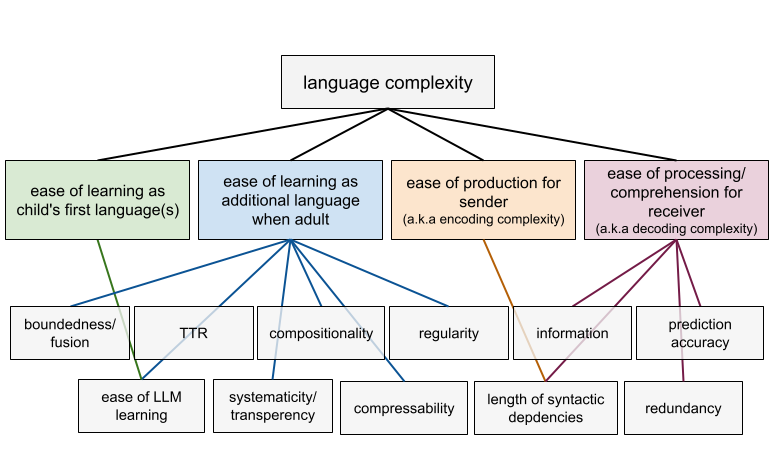
\includegraphics[width=1.2\textwidth]{latex/graphics/ud_complexity_metrics.png} % Change filename and width as needed
    \caption{Diagram of measurements of language/linguistic complexity.}
    \label{fig:metrics_diagram}
\end{figure}

In this paper, we are primarily interested in the pragmatics of information transfer between adult native speakers and how the trade-off between the encoding and decoding cost is balanced in different languages. Specifically, we are interested in variations with respect to morphological information.


%insert ackerman and malouf (2009) and Cotterell (2019) into regularity?

%Ackerman, Farrell, James P. Blevins & Robert Malouf. 2009. Parts and wholes: Implicative patterns in inflectional paradigms. In James P. Blevins & Juliette Blevins (eds.), Analogy in grammar: Form and acquisition (Oxford Linguistics), 54–82. Oxford: Oxford University Press.

%Cotterell, Ryan, Christo Kirov, Mans Hulden & Jason Eisner. 2019. On the complexity and typology of inflectional morphological systems. Transactions of the Association for Computational Linguistics 7. 327–342.


\FloatBarrier
\section{Study outline}
The aim of this study is to quantify the information in morphology annotations in corpora as a way of assessing how much information is being encoded. This can be understood as decreasing the ease of production for the sender, and thereby increasing one facet of language complexity.

Many corpora collections, such as the Universal Dependencies datasets v2.14 \citep{UD_2.14} which is used here, contain information on the morphology of individual words. Table \ref{tab:turkish_example} is an example of a sentence in Turkish where words are marked for case, number, person, aspect and more grammatical categories.
For example, the word ``horses'' in English would typically be tagged for the grammatical meaning ``plural'' being encoded morphologically.
In this study, we are not only interested in how many morphological features on average a token in a given language has - but also how informative those features are given their lemma\footnote{For this paper, we focussed on the relative frequencies of morphological features given the lemma, but it's also possible to condition on part-of-speech.}. 

\begin{table}[h]
    \centering
    \caption{Sentence 15-0000 from Universal Dependencies dataset Turkish-Penn. upos : Universal Part-of-Speech, lemma = base form, token = specific word, feats = morphological features} %note table captions go above the table
    \label{tab:turkish_example}   
    \begin{tabular}{p{1.5cm}p{2cm}p{2cm}p{6cm}}
\toprule
	\textbf{upos}	&	\textbf{lemma}	&	\textbf{token}	&	\textbf{feats}	\\
    \midrule
	ADJ	&	devasa	&	Devasa	&	\\    \midrule
	ADJ	&	ölçek	&	ölçekli	&\\    \midrule
ADJ	&	yeni	&	yeni	&		\\    \midrule
	NOUN	&	kanun	&	kanunda	&	Case=Loc|Number=Sing|Person=3	\\    \midrule
	ADJ	&	kullan	&	kullanılan	&		\\    \midrule
ADJ	&	karmaşık	&	karmaşık	&\\    \midrule
CCONJ	&	ve	&	ve	&		\\    \midrule
ADJ	&	çetrefil	&	çetrefilli	&		\\    \midrule
	NOUN	&	dil	&	dil	&	Case=Nom|Number=Sing|Person=3	\\    \midrule
	NOUN	&	kavga	&	kavgayı	&	Case=Acc|Number=Sing|Person=3|	\\    \midrule
	VERB	&	bulan	&	bulandırdı	&	Aspect=Perf|Mood=Ind|Number=Sing| Person=3|Polarity=Pos|Tense=Past| VerbForm=Fin| Voice=Cau	\\\midrule
   \multicolumn{4}{p{11cm}}{Translation: \textit{The complex and complicated language in the massive new law has muddied the fight.}}\\    \bottomrule


    \end{tabular}
\end{table}

Words can be grouped according to their lemma (base-form). 
For example ``horse'', ``horses'', ``horse's (possessive)'' all have the same lemma, usually represented in the singular, nominative non-possessive form, i.e. ``horse''.
The information stored in the morphological feature on the token can be understood as dependent on the relative frequencies of that feature on that lemma. 

For example, in the Turkish-Penn dataset of Universal Dependencies 2.14 there are 52 tokens with the lemma ``kanun'' (Eng: \textit{law}). 47 of those tokens are marked as singular for the number category, and 5 as plural. Most of the time when people use this word in this corpus, it's singular.
Were we only to know that a token has the lemma ``kanun'', we would have a good chance (90\%) to guess correctly if we said it was in the singular form.
It is possible to argue that the category of number for this lemma is not very informative, it's most often the same.
If we were to see an instance of a token with the lemma ``kanun'' with plural marking, we ought to be a bit more surprised.
Conversely, tokens for the lemma ``fiyat'' (Eng: \textit{price}) has a 55\%/45\% chance of being plural vs. singular (plural = 237, singular = 196). Were we to only know that a token was of this lemma, we'd have a harder time guessing it's number category. The number morphology for ``fiyat'' is more informative than that for ``kanun''.
This is is at the core of our metric in this paper, how informative is the morphology?



\subsection{Data}
\citet{UD_2.14}

\subsection{Similar studies}

This was for example done with the Grambank informativity metric used in \cite{grambank_release} and \citet{shcherbakova2023societies}. Given different distinctions covered in the Grambank questionnaire, say for example inclusive / exclusive or masculine / feminine pronouns, you tally up 

[STE WRITES ABOUT \citet{ccoltekin2023complexity} HERE]

\subsection{Detailed technical procedure}

[STE WRITES ABOUT OUR PROCEDURE HERE]

\subsection{Caveats}
No method is perfect. We note the shortcomings of our study here. 

\subsubsection{Comparability}
In comparative studies, it is desirable to compare like with like. There are several comparability challenges in this study. 
Datasets can for example vary in the fine-grained analysis of morphology. 
Some datasets can have contain a lot of different morphological features and some very few despite the underlying languages being similar. 
This is due to the design choices of the specific contributosr of datasets. 
In order to address this, we only consider morphological features that belong to the so called ``Universal'' feature set of the UD-project \citep{ud_2_feat_website}: Gender, Animacy, NounClass, Number, Case, Definite, Deixis, DeixisRef, Degree, VerbForm, Mood, Tense, Aspect, Voice, Evident, Polarity, Person, Polite and Clusivity.

Another comparability issue is related to genre. 

Comparability of genre across UD-treebanks

Accuracy and comparability of tokenization, UPOS, lemma and morphology feature tagging
%ud_2_feat_website

\subsubsection{Additional information}
Conditional probabilities (if Case=Nom, then Animacy=Anim more likely)
Ignoring order of elements

\subsubsection{Phonological realisation of morphological features}
Morph feats aren't attached to phonological content (or lack thereof)




\section{Results}

\section{Discussion}

\section{Conclusion}


\bibliographystyle{unified}
\bibliography{bib.bib}

	
\end{document}